\chapter{ETS}
\label{ETS}
Jedná se o konfigurační softwarový nástroj, který je nezávislý na výrobci pro navrhování, konfiguraci inteligentních instalací, a také pro řízení budov pomocí systému KNX. Tento software funguje pouze na počítačových platformách využívajících operační systém Windows. \cite{ETS Kecy}.

\noindent Pomocí softwaru lze \cite{Mitrenga}:
\begin{itemize}
    \item \textbf{Vkládat katalogové produkty do projektu} -- Produkty schválené asociací KNX jsou obsaženy v katalogu a lze je použít v projektu. Produkty lze také přidávat manuálně prostřednictvím aplikačních programů s koncovkou ".knxprod".
    \item \textbf{Vytvořit architekturu objektu} -- rozdělit objekt na celky(budovy, patra, místnosti,...)
    \item \textbf{Parametrizace produktů}
    \item \textbf{Vytváření skupinových adres}
    \item \textbf{Nahrávání řešení projektu do přístrojů}
    \item \textbf{Vzdálené ovládání připojeného projektu}
    \item \textbf{Diagnostika}
    \item \textbf{Vytvoření dokumentace}
\end{itemize}

\section{Tvorba instalace}
Při vytváření projektu byl zvolen typ páteřní linie na IP, skupinové adresy byly zvoleny třístupňové a topologie typu TP. TP topologie byla použita i při tvorbě panelu.

Po úspěšném založení projektu se program přepnul do pracovní části, která je složená z osmi oken \cite{Mitrenga}:
\begin{itemize}
    \item \textbf{Budovy} - rozdělení objektu na celky
    \item \textbf{Skupinové adresy} - vytvoření a přiřazení skupinových adres přístrojům
    \item \textbf{Topologie} - zobrazení rozložení vytvořeného projektu v topologii
    \item \textbf{Kořeny projektu} - zobrazení všech oken kde se pracovalo
    \item \textbf{Přístroje} - seznam přístojů v projektu
    \item \textbf{Zprávy} - okno zaměřené na tvorbu dokumentace projektu
    \item \textbf{Katalog} - vyhledání a vložení produktů do projektu
    \item \textbf{Diagnostika} - okno určené pro otestování instalace\\
\end{itemize}

Pro vytvoření pracovního prostoru bylo použito okno \textit{budova}. Prostor byl pojmenován \textit{Demonstrativní panel} a byl rozdělen na pět logických celků. Tyto celky reprezentují pokoje zobrazené na panelu (vchod, kuchyň, koupelna, obývací pokoj a rozvaděč umístěný v zadní části panelu). Toto rozdělení bylo vytvořeno za účelem zvýšení přehlednosti objektu a následné ulehčení propojování přístrojů mezi sebou. Je nutno také dodat, že vytvoření jedné místnosti je podmínkou pro vkládání přístrojů do pracovní plochy.

Pro vložení přístrojů bylo nutno otevřít okno katalog, který ovšem neobsahoval použité přístroje. Kvůli této komplikaci bylo nutno navštívit webové stránky výrobců a následné stažení aplikačních programů. Tyto programy byly importovány do katalogu pomocí tlačítka \textit{Import...}. Vzhled projektu po přidání přístrojů lze vidět na Obr. \ref{fig:Projekt budovy v ETS}.

\begin{figure}[!h]
  \begin{center}
    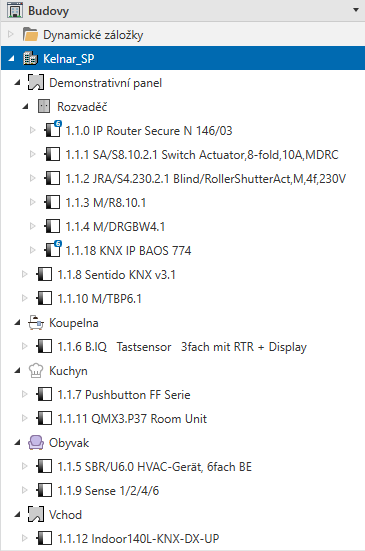
\includegraphics[scale=0.7]{obrazky/Budova.png}
  \end{center}
  \caption[Projekt budovy v ETS]{Projekt budovy v ETS}
  \label{fig:Projekt budovy v ETS}
\end{figure}

Po přidání všech přístrojů se zobrazila pracovní plocha, která slouží k zobrazení přehledu všech přístrojů (Zabezpečení - KNX Secure, individuální adresa prvku, místnost v projektu, použitý aplikační program, stav přístroje - nahrána adresa, program, parametrizace, skupinová adresa a informace o produktu). Ve sloupcích vyjadřujících stav přístroje jsou většinově pomlčky, které znázorňují, že nebyly nahrány všechny části do přístrojů. Tahle skutečnost je zdůvodněná změnami parametrů a skupinových adres.

\begin{figure}[!ht]
  \begin{center}
    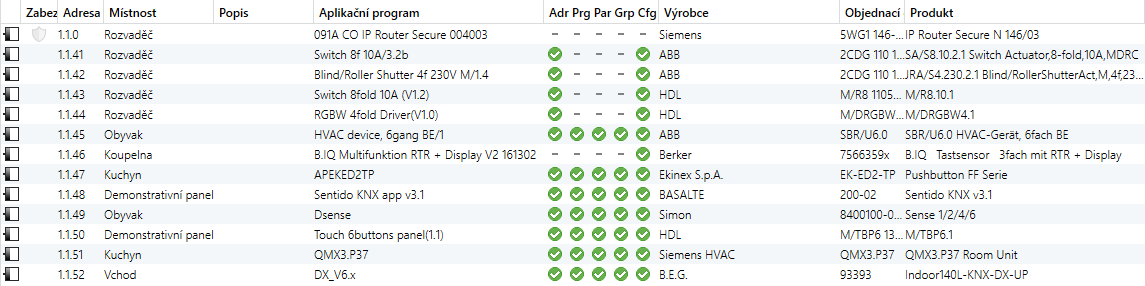
\includegraphics[scale=0.5]{obrazky/Přístroje v ETS.png}
  \end{center}
  \caption[Pracovní plocha v ETS]{Pracovní plocha v ETS}
  \label{fig:Pracovní plocha v ETS}
\end{figure}

\section{Parametrizace tlačítek a detektoru pohybu}
V této podkapitole je vysvětleno parametrizování použitých tlačítek. Ta byla pomyslně rozdělena do místností a nastavena, tak aby spolupracovala s nejbližšími prvky (světly, žaluziemi, klimatizací a topením), které jsou zobrazeny na Obr. \ref{fig:Vzheled panelu}. Pro vysvětlení byly vytvořeny tabulky popisu funkcí jednotlivých tlačítek. 

\begin{figure}[!h]
  \begin{center}
    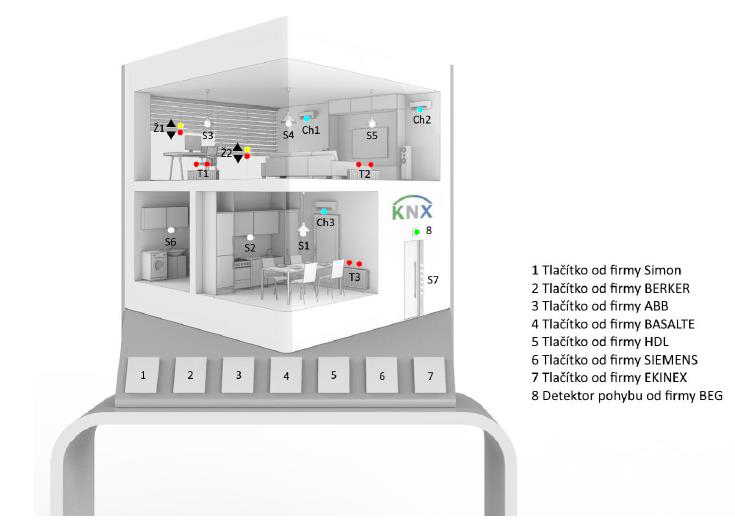
\includegraphics[scale=0.7]{obrazky/Panel_vzhled.png}
  \end{center}
  \caption[Grafický návrh panelu \cite{Mitrenga}]{Grafický návrh panelu \cite{Mitrenga}}
  \label{fig:Vzheled panelu}
\end{figure}

\subsection{ABB - SBR/U6.0.1-84}
Jedná se o šestinásobné tlačítko se zabudovaným termostatem, které lze použít na regulaci teploty, ovládání žaluzií, ovládání osvětlení a nastavení dvou scén, které mohou obsahovat až osm objektů. Každé stisknutí tlačítka změní barvu signalizační LED na předem stanovenou hodnotu (rozpoznání zapnuto/vypnuto). \cite{ABB}

\begin{figure}[!ht]
  \begin{center}
    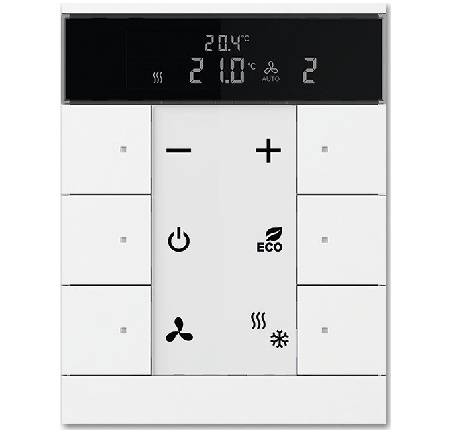
\includegraphics[scale=1.6]{obrazky/ABB.jpg}
  \end{center}
  \caption[Šestinásobné tlačítko s termostatem ABB - SBR/U6.0.1-84 \cite{ABB}]{Šestinásobné tlačítko s termostatem ABB - SBR/U6.0.1-84 \cite{ABB}}
  \label{fig:Šestinásobné tlačítko s termostatem ABB SBR/U6.0.1-84}
\end{figure}
Tlačítko bylo nastaveno na odesílání aktuální hodnoty teploty každých deset minut. Tlačítka jsou rozložena po horizontálních párech s označením funkční blok 1 až 3. V záložce každého bloku byla nastavena obě tlačítka na krátká a dlouhá stisknutí. V záložkách  \textit{Common parameter} byl vybrán typ objektu na 1-bit. Při krátkém stisknutí tlačítko odesílá hodnotu 1, při dlouhém stisknutí posílá hodnotu 2. Následně v záložce \textit{Extended parameters} byly nastaveny hodnoty odesílaných objektů u dlouhého stisknutí na on ("1") a u krátkého na off ("0").
V záložkách \textit{LED Button} pro každý funkční blok byla každá dioda nastavena do modu status. Přijímaný objekt byl nastaven na 1-bit a hodnota jasu na \textit{bright} signalizační barvu LED diod, tedy bílou při vypnutí a červenou při zapnutí. 
\subsection{Berker - 75663593}
Osminásobné tlačítko s termostatem by mělo být schopno regulovat pokojovou teplotu, ovládat žaluzie, ovládat osvětlení a scény. V této práci se ovšem nepovedlo nastavit ani při použití více zařízení a softwaru od Berkeru, který dokázal otevřít externí okno parametrizace v německém jazyce. Po ukončení parametrizace se parametry neuloží. \cite{Berker}
\begin{figure}[!ht]
  \begin{center}
    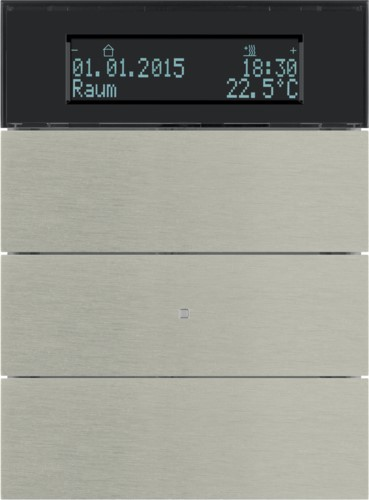
\includegraphics[scale=1.3]{obrazky/Berker.jpg}
  \end{center}
  \caption[Osminásobné tlačítko Berker - 75663593 \cite{Berker}]{Osminásobné tlačítko - Berker - 75663593 \cite{Berker}}
  \label{fig:Osminásobné člačítko s termostatem Berker 75663593}
\end{figure}
\newpage
\subsection{Ekinex - EK-ED2-TP-RW}
Jedná se o čtyřnásobné tlačítko se zabudovaným teplotním senzorem pro ovládání žaluzií, osvětlení a scén. \cite{Ekinex}

\begin{figure}[!ht]
  \begin{center}
    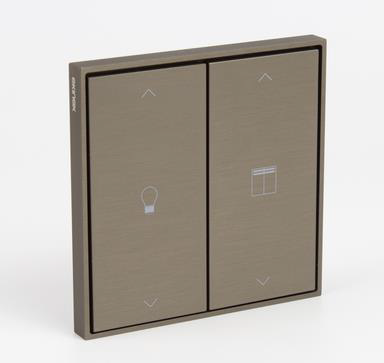
\includegraphics[scale=0.6]{obrazky/Ekinex.png}
  \end{center}
  \caption[Čtyřnásobné tlačítko Ekinex - EK-ED2-TP-RW \cite{Mitrenga}]{Čtyřnásobné tlačítko Ekinex - EK-ED2-TP-RW \cite{Mitrenga}}
  \label{fig:Čtyřnásobné tlačítko se zabudovaným teplotním senzorem Ekinex - EK-ED2-TP-RW}
\end{figure}

Tlačítko bylo nastaveno v záložce \textit{General} na dvě svislé klapky. Obě klapky byly nastaveny na dlouhé a krátké stisknutí. V případě první klapky se horní krátký stisk nastavil na funkci \textit{toggle} (přepínání). Dlouhý stisk představuje funkci \textit{off}. Pro dolní část klapky, je nastavení přesně opačné. Druhá klapka je nastavená stejným způsobem, akorát místo funkce \textit{toggle} byla použita funkce \textit{none}. Tato funkce zasílá "0", což znamená u žaluzií pohyb směrem nahoru.

\subsection{Basalte - Senido 202-03}
Další z použitých snímačů je čtyřnásobné dotykové tlačítko se zabudovaným snímačem teploty pro ovládání žaluzií, osvětlení a scén. Toto tlačítko má rovněž schopnost rozlišovat krátké a dlouhé stisknutí, a to nejen na jednom segmentu, ale má možnost snímat více segmentů najednou (multitouch). Dokáže ovládat až šest scén s osmi objekty. Další ze schopností tlačítka je posílání tříbajtové hodnoty RGB. Poslední z funkcí tlačítka je zobrazování statusu díky RGB podsvícení. \cite{Basalte}

\begin{figure}[!ht]
  \begin{center}
    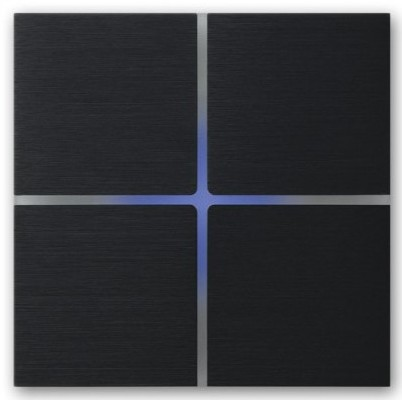
\includegraphics[scale=0.4]{obrazky/Basalte.jpg}
  \end{center}
  \caption[Čtyřnásobné dotykové tlačítko Basalte - Senido 202-03 \cite{Basalte}]{Čtyřnásobné dotykové tlačítko Basalte - Senido 202-03 \cite{Basalte}}
  \label{fig:Čtyřnásobné dotykové tlačítko Basalte - Senido 202-03}
\end{figure}

Tlačítko bylo rozděleno na čtyři samostatné zóny v záložce \textit{General}. Dále se v této záložce povolila funkce řadiče scén. První trojici tlačítek byla nastavena scéna, kterou budou při stisknutí volat.  Každá z těchto scén byla nastavena v korespondující záložce označené číslem. Poslední tlačítko bylo nastaveno na demonstraci schopnosti zasílat hodnoty RGB. Jedná se o 2 nastavené hodnoty, které se rozlišují délkou stisku. Pro demonstraci funkce multitouch byla vybrána funkce \textit{room toggle + General on/off/scene}. Pro krátký stisk byla vybrána scéna, která se zapne při krátkém stisku. Při druhém stisku se panel vypne. Dlouhý stisk má přiřazenou vlastní scénu. V záložce \textit{Temperature senzor} bylo nastaveno, aby senzor zasílal teplotu každých 5 minut. Záložka \textit{Scene controller}, která je určená pro nastavení řadiče scén, byla nastavena na všech výstupech na hodnotu 1-bit.

\subsection{Simon - 8400100-039}
Čtyřnásobné tlačítko se zabudovaným RGB podsvícením a teplotním senzorem pro ovládání žaluzií a osvětlení. \cite{Simon}

\begin{figure}[!ht]
  \begin{center}
    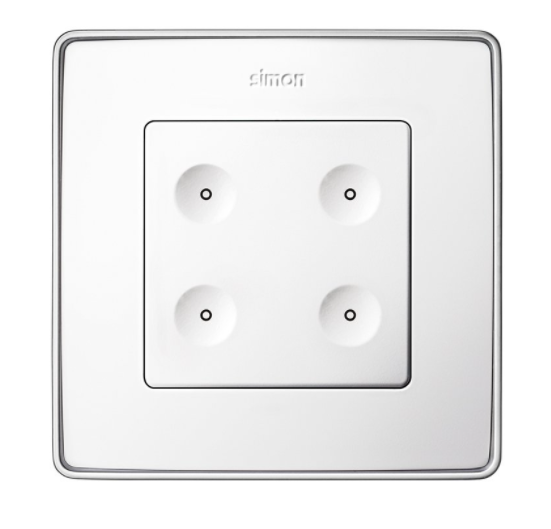
\includegraphics[scale=0.4]{obrazky/Simon.png}
  \end{center}
  \caption[Čtyřnásobné tlačítko Simon - 8400100-039 \cite{Simon}]{Čtyřnásobné tlačítko Simon - 8400100-039 \cite{Simon}}
  \label{fig:Čtyřnásobné tlačítko Simon - 8400100-039}
\end{figure}

V záložce \textit{General} bylo vybráno čtyř tlačítkové provedení, které je použito na demonstrativním panelu. Jako další možnost, která byla povolena, byl vnitřní senzor teploty. Poté v záložce \textit{FeedBack} byly nastaveny hodnoty jasu a hlasitosti na maximum. Dále zde byla aktivována možnost zpětné vazby doteku vibracemi. Pro nastavení samotné funkcionality tlačítek se musela použít záložka \textit{Inputs}, kde se nastavilo oddělení tlačítek od sebe (všechna tlačítka jsou samostatně). Tlačítka v tomto případě jsou číslována od spodního levého rohu po sloupcích (1 a 2 levá strana, 3 a 4 pravá strana). Poté už se nastavovala samotná funkcionalita tlačítek. Byla vybrána možnost krátkého i dlouhého stisku. V případě krátkého stisku žaluzie vyjedou/sjedou samostatně. Dlouhý stisk znamená pohyb pouze v čase, kdy je tlačítko stisknuto.

\subsection{HDL - M/TBP6.1-A2}
Předposlední tlačítko je od společnosti HDL. Jedná se o šestinásobné dotykové tlačítko se zabudovaným RGB podsvícením pro ovládání žaluzií, osvětlení, stmívání a ovládání dvou scén s deseti objekty. Dále také obsahuje RGB kontrolér, který dokáže posílat 3-byte hodnotu obsahující informace o intenzitě každé složky. \cite{HDL}

\begin{figure}[!ht]
  \begin{center}
    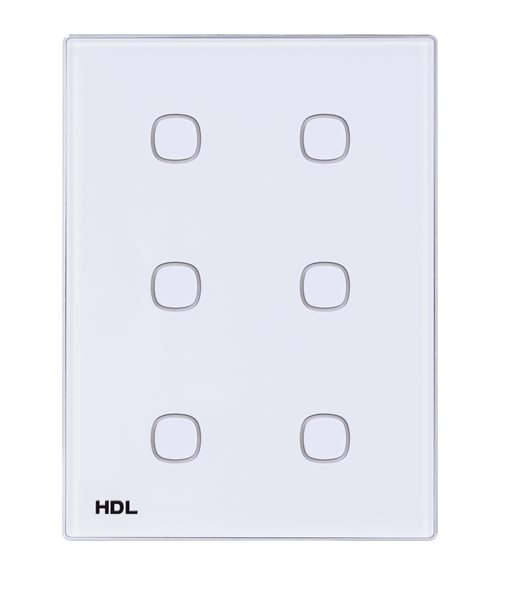
\includegraphics[scale=0.25]{obrazky/HDL.jpg}
  \end{center}
  \caption[Šestinásobné tlačítko HDL - M/TBP6.1-A2 \cite{HDL}]{Šestinásobné tlačítko HDL - M/TBP6.1-A2 \cite{HDL}}
  \label{fig:Šestinásobné tlačítko HDL - M/TBP6.1-A2}
\end{figure}

\newpage První z parametrů, které je možno nastavit v záložce \textit{General} byla citlivost dotyku, a to na hodnotu 4. Dále se pak povolily scény. Následně se obě scény nastaví v záložkáckách \textit{Panel scene A} a \textit{Panel scene B}. První scéna byla nastavena dle Obr. \ref{fig:Parametry scény A tlačítka HDL - M/TBP6.1-A2} a druhá dle Obr. \ref{fig:Parametry scény B tlačítka HDL - M/TBP6.1-A2}.

\begin{figure}[!ht]
  \begin{center}
    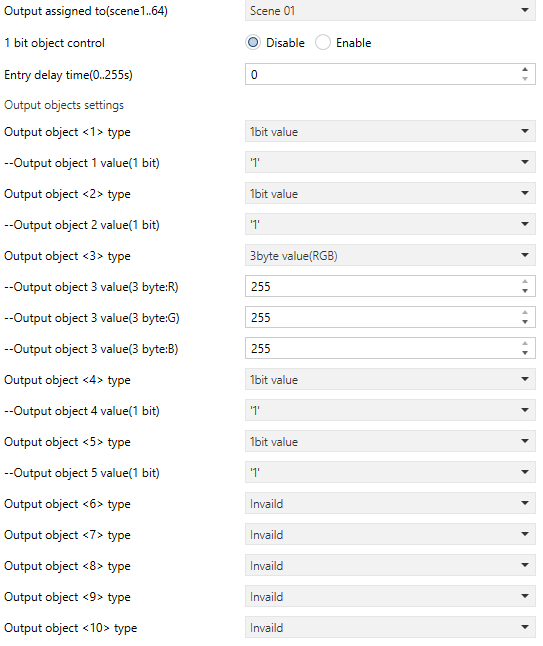
\includegraphics[scale=0.4]{obrazky/Scena A.png}
  \end{center}
  \caption[Parametry scény A tlačítka HDL - M/TBP6.1-A2]{Parametry scény A tlačítka HDL - M/TBP6.1-A2}
  \label{fig:Parametry scény A tlačítka HDL - M/TBP6.1-A2}
\end{figure}

\begin{figure}[!ht]
  \begin{center}
    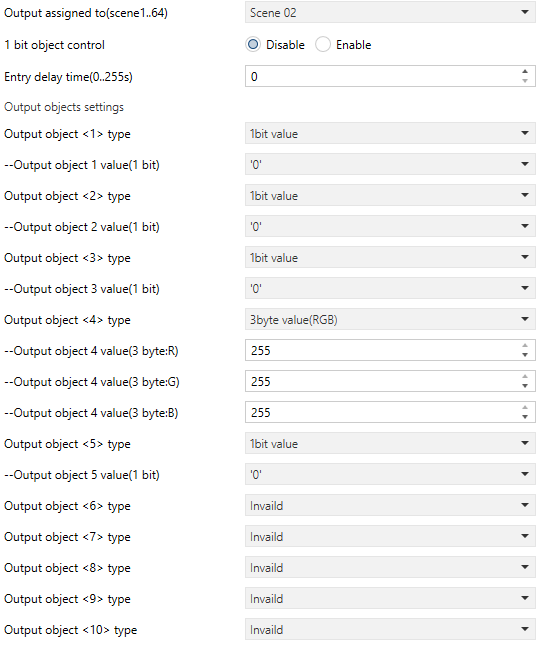
\includegraphics[scale=0.4]{obrazky/Scena B.png}
  \end{center}
  \caption[Parametry scény B tlačítka HDL - M/TBP6.1-A2]{Parametry scény B tlačítka HDL - M/TBP6.1-A2}
  \label{fig:Parametry scény B tlačítka HDL - M/TBP6.1-A2}
\end{figure}

Každé z těchto tlačítek má nastaveno signaliční podsvícení na jinou hodnotu. Krátkému stisknutí byla přiřazena funkce \textit{toggle}, která dovoluje přepínat osvětlení mezi hodnotami zapnuto a vypnuto. Dlouhé stisknutí bylo nastaveno na dobu 1s a používá se na stmívání. Pro demonstraci stmívání byly nastaveny různé hodnoty kroku prvních 4 tlačítek. Každé z těchto tlačítek má nastavenou signaliční podsvícení na jinou hodnotu. První tlačítko bylo nastaveno červenou barvu, druhou na zelenou, třetí na modrou a čtvrté na bílou. Při signalizaci se zvýší jas barev o 70\%. Zbylá 2 tlačítka byla přepnuta do modu RGB kontrolér, který odesílají hodnotu RGB jak pro krátké, tak i pro dlouhé stisknutí. Tato hodnota se také signalizuje při stisknutí tlačítek. 

\subsection{Siemens - QMX3.P37}
Jedná se o ovládací panel určený na regulování pokojové teploty s integrovaným displejem. Tento displej dokáže zobrazovat vlhkost vzduchu, koncentraci CO2 v ovzduší a samotnou teplotu místnosti. Také obsahuje osm tlačítek, která obsahují žluté statusové LED. Tento panel umožňuje také ovládání žaluzií, osvětlení a scény. \cite{Siemens}

\begin{figure}[!ht]
  \begin{center}
    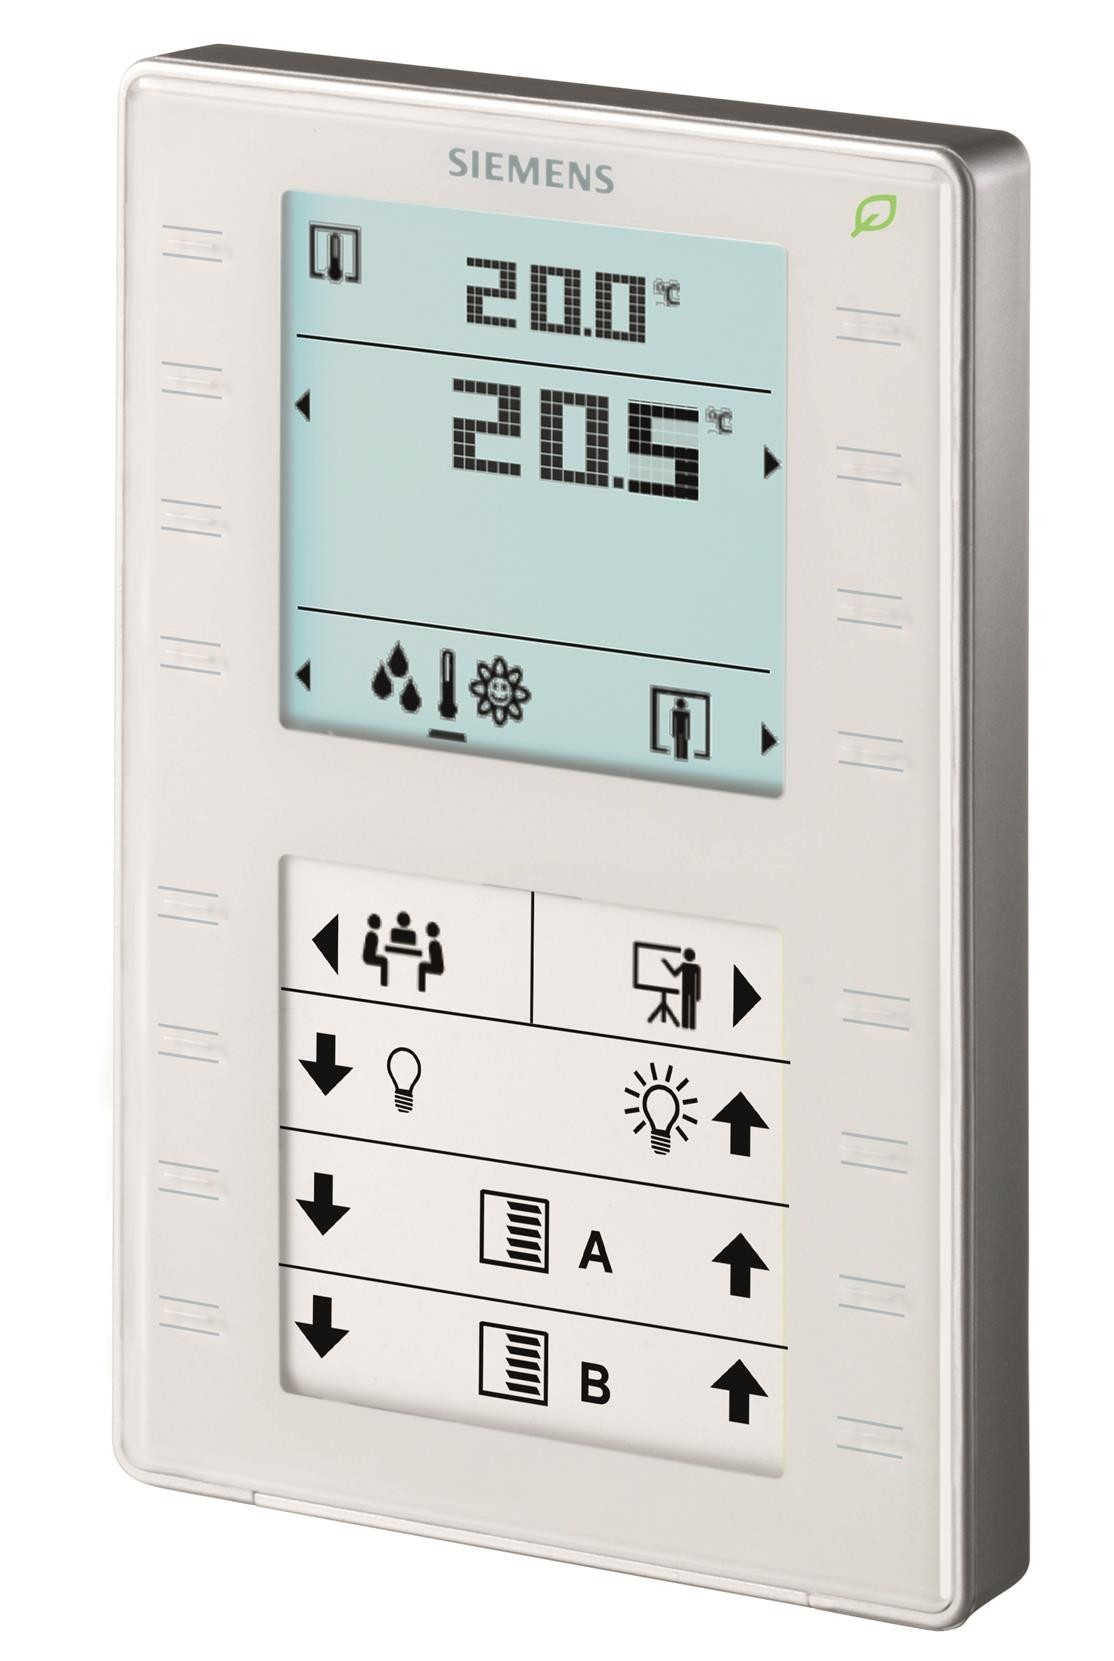
\includegraphics[scale=0.125]{obrazky/Siemens.jpg}
  \end{center}
  \caption[Ovladací panel Siemens - QMX3.P37 \cite{Siemens}]{Ovladací panel Siemens - QMX3.P37 \cite{Siemens}}
  \label{fig:Ovladací panel Siemens - QMX3.P37}
\end{figure}

V tomto případě bylo zařízení nastaveno na spínání pomocí jednoho tlačítka. Nejprve v záložce \textit{General} byla nastavena hodnota svitu signaližačnních LED na 100\% hodnotu. V další záložce byl nastaven teplotní senzor na odesílání hodnoty každých 10 minut. Poté se už nastavovaly jednotlivé tlačítkové páry. Funkce páru byla zvolena \textit{Individual}, která umožňuje nezávislé fungování obou tlačítek. Dále se u obou tlačítek nastavila možnost \textit{1 - button switching / send value}, \textit{Short/long press} (dlouhé stisknutí po uplynutí půl sekundy) a vybrala se možnost odesílání druhé hodnoty při dlouhém stisku. Levým tlačítkům byla přiřazena hodnota \textit{on} a pravým \textit{off}. Také byla nastavena signalizace stisku tlačítek. Kvůli tomu byla možnost \textit{LED display} nastavena na \textit{status object} a možnost \textit{LED activation} pro levá tlačítka na \textit{0 = LED off; 1 = LED on}. Pravá tlačítka byla nastavena \textit{0 = LED on; 1 = LED off}. Po pozdější úvaze o zefektivnění panelu se pro 1. a 4. řadu tlačítek změnil dlouhý stisk na \textit{Toggle}.  

\subsection{B.E.G - Indor 140-L-KNX-DX}
V první záložce \textit{Grundeinstellungen} (Základní nastavení) se nastavila hodnota teploměru (Temperaturmessung) na aktiviert. \cite{BEG}

Parametrizace tohoto prvku byla celá v němčině, a to dosti zkomplikovalo postup. První záložka \textit{Grundeinstellungen} (Základní nastavení) se nastavila hodnota teploměru (Temperaturmessung) na aktiviert. Poté v záložce teploměru se v možnosti zasílání teploty (\textit{Temperaturwer senden}) zvolilo odesílání při změně (bei Änderung). Další parametry byly nastaveny v záložce \textit{Tastenfunktionen} (Klíčové funkce), kde se aktivovala tlačítka T1 a T2. Nastavení \textit{Präsenzmelder} (Detektor pohybu) zůstalo v plně automatickém řežimu (\textit{Vollautomatik}). V první podzáložce detektoru pohybu byla nastavená doba vypnutí na 30 sekund. Při nastavování obou tlačítek byl vybrán režim spínání (\textit{Betriebsart}).

\begin{figure}[!ht]
  \begin{center}
    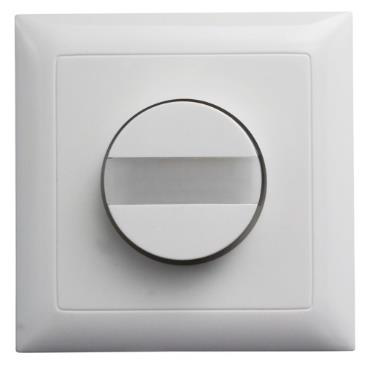
\includegraphics[scale=0.45]{obrazky/BEG.png}
  \end{center}
  \caption[Detektor pohybu B.E.G - Indor 140-L-KNX-DX \cite{Mitrenga}]{Detektor pohybu B.E.G - Indor 140-L-KNX-DX  \cite{Mitrenga}}
  \label{fig:Detektor pohybu B.E.G - Indor 140-L-KNX-DX }
\end{figure}

\section{Parametrizace akčních členů}
Tahle podkapitola se zaměřuje na parametrizaci použitých akčních členů umístěných v rozvaděči na zadní straně panelu.
\subsection{ABB SA/S8.10.2.1}
Tento osmikanálový spínací člen nebyl nijak parametrizován a byl ponechán ve stavu spínacího aktoru, který zasílá status pouze při změně. Úkolem tohoto aktoru je spínání LED představující topení a klimatizaci.

\begin{figure}[!ht]
  \begin{center}
    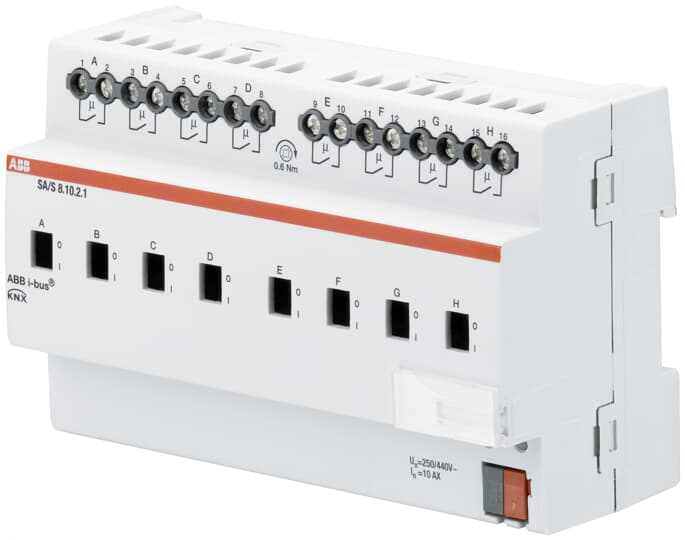
\includegraphics[scale=0.25]{obrazky/ABB aktor1.jpg}
  \end{center}
  \caption[Osmikanálový spínací člen ABB - SA/S8.10.2.1 \cite{ABB aktor1}]{Osmikanálový spínací člen ABB - SA/S8.10.2.1  \cite{ABB aktor1}}
  \label{fig:Osmikanálový spínací člen ABB - SA/S8.10.2.1}
\end{figure}

\subsection{ABB - JRA/S4.230.2.1}
Jedná se o čtyřkanálový žaluziový člen, který je určen k ovládaní žaluzií. Jelikož se v projektu používají pouze 2 žaluziové okruhy, tak se využívá pouze polovina akčního členu. Využívají se první dva kanály. Jediná změna od původní parametrizace je v záložkách \textit{Drive} pro jednotlivé kanály a to nastavení ukončení pohybu po 5 sekundách (tj. žaluzie může po stisku vyjíždět/sjíždět po dobu maximálně 5 sekund). 

\begin{figure}[!ht]
  \begin{center}
    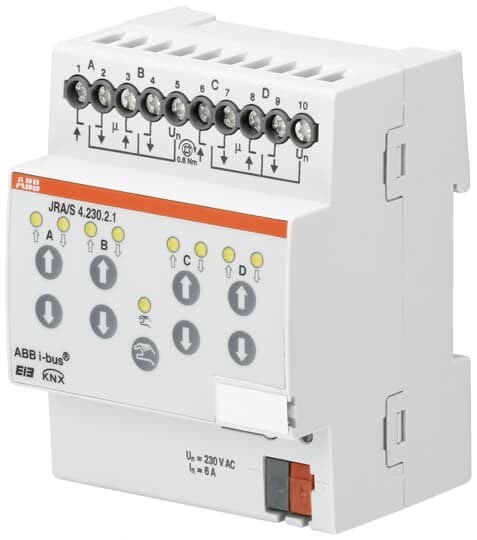
\includegraphics[scale=0.25]{obrazky/ABB aktor2.jpg}
  \end{center}
  \caption[Čtyřkanálový žaluziový člen ABB - JRA/S4.230.2.1 \cite{ABB aktor2}]{Čtyřkanálový žaluziový člen ABB - JRA/S4.230.2.1  \cite{ABB aktor2}}
  \label{fig:Čtyřkanálový žaluziový člen ABB - JRA/S4.230.2.1}
\end{figure}

\subsection{HDL - M/R8.10.1}
Osmikanálový spínací člen HDL se v této práci využívá ke spínání osvětlení tedy 7 LED, které představují osvětlení umístěné v domě. V tomto případě nebyla nutná žádná změna oproti původnímu nastavení parametrů. Všechny kanály jsou nastaveny jako spínací aktor s typem kontaktu Normally Opened (NO). Zasílání statusu probíhá pouze při změně hodnoty.

\begin{figure}[!ht]
  \begin{center}
    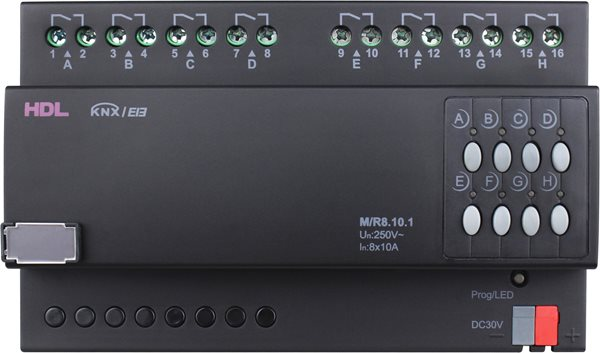
\includegraphics[scale=0.35]{obrazky/HLD aktor1.jpg}
  \end{center}
  \caption[Osmikanálový spínací člen HDL - M/R8.10.1 \cite{HDL aktor1}]{Osmikanálový spínací člen HDL - M/R8.10.1  \cite{HDL aktor1}}
  \label{fig:Osmikanálový spínací člen HDL - M/R8.10.1}
\end{figure}

\subsection{HDL - M/DRGBW4.1}
Čtyřnásobný stmívací člen poskytnutý společností HDL byl v této práci použit na ovládání RGBW LED pásku ukrytém v demonstrativním panelu. Výhodou tohoto členu je možnost ovládat kanál barevných složek zvlášť. Každý kanál (\textit{Channel}) je nastaven na odesílání stavové hodnoty (1bit) při změně. Dále se nastavily hodnoty času pro stmívání v záložkách \textit{dimming config} každého kanálu na 1 sekundu pro zapnutí i vypnutí. 

\begin{figure}[!ht]
  \begin{center}
    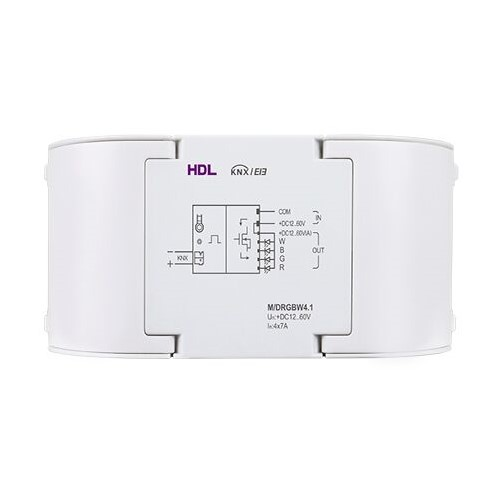
\includegraphics[scale=0.4]{obrazky/HLD aktor2.jpg}
  \end{center}
  \caption[Čtyřnásobný stmívací člen HDL - M/DRGBW4.1 \cite{HDL aktor2}]{Čtyřnásobný stmívací člen HDL - M/DRGBW4.1 \cite{HDL aktor2}}
  \label{fig:Čtyřnásobný stmívací člen HDL - M/DRGBW4.1}
\end{figure}

\section{Připojená komunikační rozhraní}
Pro umožnění parametrizace a externího řízení bylo nutno přidat do projektu dvě různá rozhraní pro komunikaci. První z nich je IP Secure router Siemens - 5WG1 146-1AB03, který je převážně určen k bezpečnému přenosu dat. Lze z něj také vytvořit liniovou spojku. \cite{Siemens IP}

Tomuto rozhraní byla pouze nastavena IP adresa, maska a základní brána pro komunikaci s RaspberryPi skrze tunelování.

\begin{figure}[!ht]
  \begin{center}
    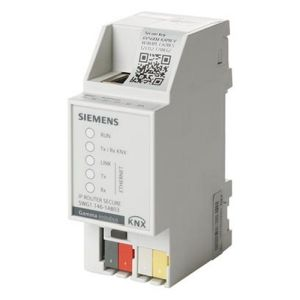
\includegraphics[scale=0.55]{obrazky/Siemens router.jpg}
  \end{center}
  \caption[IP Secure router Siemens - 5WG1 146-1AB03 \cite{Siemens IP}]{IP Secure router Siemens - 5WG1 146-1AB03 \cite{Siemens IP}}
  \label{fig:IP Secure router Siemens - 5WG1 146-1AB03}
\end{figure}

Druhé komunikační rozhraní použité na panelu je Weinzierl - KNX IP BAOS 774. Využívá se pro komunikaci skrze telegramy nebo datové body. Dále umožňuje přístup k objektům pomocí TCP/IP protokolu anebo za pomoci webového rozhraní. \cite{Weinzier}

Toto rozhraní bylo taktéž parametrizováno pro komunikaci s PLC. Byla mu nastavena odlišná IP adresa, stejná maska a brána jako u předchozího rozhraní. Dále se v něm definovaly datapointy pro komunikaci. Ty jsou definované v tabulce \ref{tab:Datapointy pro komunikaci KNX IP BAOS 774 s PLC}.

\begin{figure}[!ht]
  \begin{center}
    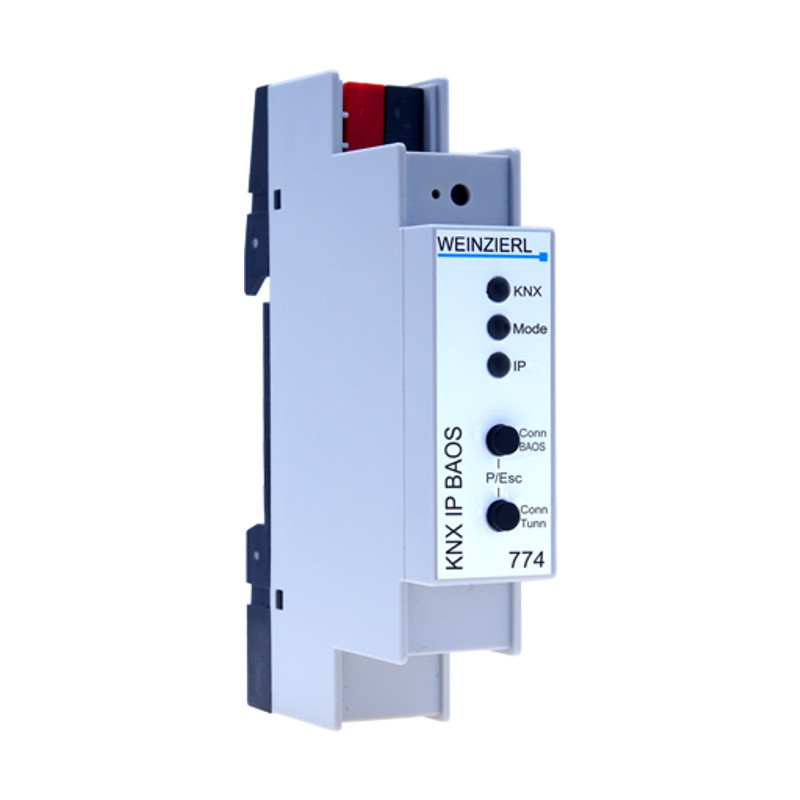
\includegraphics[scale=0.2]{obrazky/IP BAOS.jpg}
  \end{center}
  \caption[Komunikační rozhraní Weinzierl - KNX IP BAOS 774 \cite{Weinzier ob}]{Komunikační rozhraní Weinzierl - KNX IP BAOS 774 \cite{Weinzier ob}}
  \label{fig:Komunikační rozhraní Weinzierl - KNX IP BAOS 774}
\end{figure}
\pagebreak
\begin{table}[!ht]
  \caption[Datapointy pro komunikaci KNX IP BAOS 774 s PLC]{Datapointy pro komunikaci KNX IP BAOS 774 s PLC}
  \label{tab:Datapointy pro komunikaci KNX IP BAOS 774 s PLC}
  \small
    \centering
    \begin{tabular}{|c|c|c|}
      \hline
        Datapoint & Typ & Účel  \\
          \hline\hline
            1. & DPT 1 & Světlo pracovna zpětná vazba \\
          \hline
            2. & DPT 1 & Světlo obývací pokoj zpětná vazba \\
          \hline
            3. & DPT 1 & Světlo televize zpětná vazba \\
          \hline
            4. & DPT 1 & Světlo linka zpětná vazba \\
          \hline
            5. & DPT 1 & Světlo kuchyně zpětná vazba \\
          \hline
            6. & DPT 1 & Světlo koupelna zpětná vazba \\
          \hline
            7. & DPT 1 & Vchodové světlo zpětná vazba \\
          \hline
            8. & DPT 1 & Topení pracovna zpětná vazba \\
          \hline
            9. & DPT 1 & Topení televize zpětná vazba \\
          \hline
            10. & DPT 1 & Topení kuchyň zpětná vazba \\
          \hline
            11. & DPT 1 & Klimatizace pracovna zpětná vazba \\
          \hline
            12. & DPT 1 & Klimatizace televize zpětná vazba \\
          \hline
            13. & DPT 1 & Klimatizace kuchyně zpětná vazba \\
          \hline
            14. & DPT 1 & Levé žaluzie zpětná vazba \\
          \hline
            15. & DPT 1 & Levé žaluzie příkaz \\
          \hline
            16. & DPT 1 & Pravé žaluzie zpětná vazba \\
          \hline
            17. & DPT 1 & Pravé žaluzie příkaz \\
          \hline
            18. & DPT 1 & Světlo pracovna příkaz \\
          \hline
            19. & DPT 1 & Světlo obývací pokoj příkaz \\
          \hline
            20. & DPT 1 & Světlo televize příkaz \\
          \hline
            21. & DPT 1 & Světlo linka příkaz \\
          \hline
            22. & DPT 1 & Světlo kuchyně příkaz \\
          \hline
            23. & DPT 1 & Světlo koupelna příkaz \\
          \hline
            24. & DPT 1 & Vchodové světlo příkaz \\
          \hline
            25. & DPT 1 & Topení pracovna příkaz \\
          \hline
            26. & DPT 1 & Topení televize příkaz \\
          \hline
            27. & DPT 1 & Topení kuchyň příkaz \\
          \hline
            28. & DPT 1 & Klimatizace pracovna příkaz \\
          \hline
            29. & DPT 1 & Klimatizace televize příkaz \\
          \hline
            30. & DPT 1 & Klimatizace kuchyně příkaz \\
          \hline
            31. & DPT 1 & Krokování levé žaluzie \\
          \hline
            32. & DPT 1 & Krokování levé žaluzie \\
          \hline
            33. & DPT 18 & Scéna odchod \\
          \hline
            34. & DPT 9 & Teplota okolí panelu \\
          \hline
  \end{tabular}
\end{table}
\newpage
\section{Vytvoření skupinových adres projektu}
V závislosti na informacích obsažených v podkapitole \ref{Adresování} se tato podkapitola zaměří pouze na tvorbu skupinových adres. První část této podkapitoly bude věnována vytvoření a popsání tabulek jednotlivých místností. Tyto tabulky budou použity pro popis funkce jednotlivých tlačítek a následně pro tvorbu skupinových adres. Dále tyto tabulky nebudou obsahovat tlačítko společnosti Berker, které nelze parametrizovat.

První místnosti, které budou nastaveny, jsou kuchyně a koupelna. Do těchto prostor byly pomyslně nainstalovány tlačíka společnosti Ekinex a Siemens. Aby se využilo maximálně těchto tlačítek, budou využita obě tlačítka i v jiných místnostech. Zejména se jedná o tlačítko Ekinex, které má na pravé klapce žaluzie. V případě tlačítka Siemens se jedná pouze o využití velkého množství tlačítek, které budou použity při dlouhém stisku na ovládání celé budovy. 

\begin{table}[h]
 \caption[Funkce kuchyňských tlačítek pro krátké stisknutí]{Funkce kuchyňských tlačítek pro krátké stisknutí}
   \small
    \centering
	  \begin{tabular}{|c|c|c|}
	    \hline
	    Tlačítko & Ekinex & Siemens  \\
	    \hline\hline
	    1. & S1 Zapnuto/Vypnuto & Ch3 Vypnuto \\
	    \hline
        2. & S2 Zapnuto/Vypnuto & Ch3 Zapnuto \\
	    \hline
        3. & Ž1, Ž2 krok nahorů & T3 Vypnuto \\
	    \hline
        4. & Ž1, Ž2 krok dolů & T3 Zapnuto \\
	    \hline
        5. & - & T3/1 Vypnuto \\
	    \hline 
        6. & - & T3/1 Zapnuto \\
	    \hline 
	    7. & - & T3/2 Vypnuto \\
	    \hline
	    8. & - & T3/2 Zapnuto \\
	    \hline
	  \end{tabular}
\end{table}

\begin{table}[h]
 \caption[Funkce kuchyňských tlačítek při dlouhém stisknutí]{Funkce kuchyňských tlačítek při dlouhém stisknutí}
   \small
    \centering
	  \begin{tabular}{|c|c|c|}
	    \hline
	    Tlačítko & Ekinex & Siemens  \\
	    \hline\hline
	    1. & S1, S2, S6 Zapnuto/Vypnuto &  Ch1 Zapnuto/Vypnuto \\
	    \hline
        2. & S6 Zapnuto/Vypnuto &  Ch2 Zapnuto/Vypnuto \\
	    \hline
        3. &  Ž1, Ž2 nahorů & T1, T2, T2 Vypnuto \\
	    \hline
        4. & Ž1, Ž2 dolů & T1, T2, T2 Zapnuto \\
	    \hline
        5. & - &  Ch1, Ch2, Ch3 Vypnuto\\
	    \hline 
        6. & - & Ch1, Ch2, Ch3 Zapnuto \\
	    \hline 
	    7. & - & S1,S2,S6 Vypnuto \\
	    \hline
	    8. & - & S3,S4,S5 Zapnuto \\
	    \hline
	  \end{tabular}
\end{table}

\newpage Další místností se dvěma pomyslně nainstalovanými tlačítky je obývací pokoj. Jedná se o tlačítka společnosti ABB a Simon. Tlačítko Simon bude použito na ovládání žaluzií a tlačítko ABB na ovládání topení, chlazení a světel v místnosti.

\begin{table}[h]
 \caption[Funkce tlačítek obývacího pokoje při krátké stisknutí]{Funkce tlačítek obývacího pokoje při krátké stisknutí}
   \small
    \centering
	  \begin{tabular}{|c|c|c|}
	    \hline
	    Tlačítko & ABB & Simon  \\
	    \hline\hline
	    1. & T1 Vypnuto & Ž1 krok nahorů  \\
	    \hline
        2. & T2 Vypnuto & Ž1 krok dolů  \\
	    \hline
        3. & Ch1,Ch2 Vypnuto & Ž2 krok nahorů  \\
	    \hline
        4. & S3 Vypnuto & Ž2 krok dolů  \\
	    \hline
        5. & S4 Vypnuto & - \\
	    \hline 
        6. & S5 Vypnuto & - \\
	    \hline 
	  \end{tabular}
\end{table}

\begin{table}[h]
 \caption[Funkce tlačítek obývacího pokoje při dlouhém stisknutí]{Funkce tlačítek obývacího pokoje při dlouhém stisknutí}
   \small
    \centering
	  \begin{tabular}{|c|c|c|}
	    \hline
	    Tlačítko & ABB & Simon  \\
	    \hline\hline
	    1. & T1 Zapnuto & Ž1 nahorů  \\
	    \hline
        2. & T2 Zapnuto & Ž1 dolů  \\
	    \hline
        3. & Ch1,Ch2 Zapnuto & Ž2 nahorů  \\
	    \hline
        4. & S3 Zapnuto & Ž2 dolů  \\
	    \hline
        5. & S4 Zapnuto & - \\
	    \hline 
        6. & S5 Zapnuto & - \\
	    \hline 
	  \end{tabular}
\end{table}

Dotyková tlačítka společností Basalte a HDL byla určena na ovládání scén a barvy pozadí objektu. Tlačítko společnosti basalte v této práci reaguje pouze na  krátký dotek jednotlivých tlačítek. Tato skutečnost je způsobena použitím scén. Při použití funkce volání scény nelze využít dlouhého doteku. Další z vlastností tlačítka je již zmiňovaný multitouch, který funguje na bázi doteku dvou a více ploch najednou. V této práci je použit krátký dotek na zavolání scény odchod a dlouhý dotek na volání scény příchod.
\newpage
\begin{table}[!ht]
 \caption[Funkce dotykových tlačítek při krátké stisknutí]{Funkce dotykových tlačítek při krátké stisknutí}
   \small
    \centering
	  \begin{tabular}{|c|c|c|}
	    \hline
	    Tlačítko & Basalte & HDL \\
	    \hline\hline
	    1. & Scéna dovolená  & Červené podsvícení \\
	    \hline
        2. & Scéna léto  &  Zelené podsvícení \\
	    \hline
        3. & Scéna zima  & Modré podsvícení   \\
	    \hline
        4. & RGB Kontroler & Bílé podsvícení \\
	    \hline
        5. & - & Nastavená hodnota RGB 1 \\
	    \hline 
        6. & - &  Nastavená hodnota RGB 2 \\
	    \hline 
	  \end{tabular}
\end{table}

\begin{table}[!ht]
 \caption[Funkce dotykových tlačítek při dlouhém stisknutí]{Funkce dotykových tlačítek při dlouhém stisknutí}
   \small
    \centering
	  \begin{tabular}{|c|c|c|}
	    \hline
	    Tlačítko & Basalte & HDL  \\
	    \hline\hline
	    1. & - & Červené podsvícení stmívání  \\
	    \hline
        2. & - & Zelené podsvícení stmívání \\
	    \hline
        3. & - & Modré podsvícení stmívání  \\
	    \hline
        4. & - & Bílé podsvícení  stmívání \\
	    \hline
        5. & - & Nastavená hodnota RGB 3 \\
	    \hline 
        6. & - & Nastavená hodnota RGB 4 \\
	    \hline 
	  \end{tabular}
\end{table}

Poslední z použitých spínačů je detektor pohybu, kterému bylo logicky přiřazeno přední světlo domu.\\ \\Ze vzniklých tabulek byly vytvořeny skupinové adresy, které byly rozděleny do skupin dle přístroje (Světla, Žaluzie, Topení, Klimatizace, LED, Scény a Měření). Tyto skupiny se dále dělí podle funkcionality a množství. Poslední vrstva již představuje jednotlivé objekty nebo scény. Výpis skupinových adres je součástí příloh.